\chapter{การแปลงและปรับแต่งโมเดลสู่สถาปัตยกรรม Edge AI}
\label{chap:edge_optimization}
\index{Edge AI}
\index{ONNX Export}
\index{Quantization}

\section*{แผนบริหารการสอนประจำบทที่ 6}
\addcontentsline{toc}{section}{แผนบริหารการสอนประจำบทที่ 6}

\begin{planbox}{หัวข้อเนื้อหาประจำบท (Lesson Topics)}
\begin{enumerate}[leftmargin=1.5em, itemsep=2pt]
    \item ข้อจำกัดของฮาร์ดแวร์ประมวลผลบนขอบ (Edge Hardware Constraints) ในแปลงเกษตร
    \item สถาปัตยกรรม TorchScript และการทำ Just-In-Time (JIT) Tracing
    \item มาตรฐานเปิด Open Neural Network Exchange (ONNX) และ ONNX Runtime
    \item ทฤษฎีการลดทอนความแม่นยำตัวเลข (Quantization): จาก FP32 สู่ INT8
    \item การคำนวณค่า Scale และ Zero-Point ในกระบวนการ Quantization
    \item การตรวจสอบความถูกต้องเชิงตัวเลข (Numerical Parity Validation) ระหว่าง PyTorch และ ONNX
    \item โค้ดตัวอย่าง: สคริปต์ส่งออกและตรวจสอบโมเดล \texttt{export\_edge.py}
    \item ตัวอย่างและกรณีศึกษา: การเปรียบเทียบความเร็วและการใช้พลังงานบนฮาร์ดแวร์ 4 ชนิด
\end{enumerate}
\end{planbox}

\begin{planbox}{วัตถุประสงค์เชิงพฤติกรรม (Behavioral Objectives)}
เมื่อศึกษาบทที่ 6 จบแล้ว ผู้เรียนและผู้อ่านสามารถ:
\begin{enumerate}[leftmargin=1.5em, itemsep=2pt]
    \item อธิบายข้อแตกต่างระหว่างรูปแบบไฟล์โมเดล PyTorch (.pth), TorchScript (.pt) และ ONNX (.onnx) ได้
    \item คำนวณค่า Scale Factor และ Zero-Point สำหรับการแปลงข้อมูล FP32 เป็น INT8 ได้อย่างถูกต้อง
    \item เขียนสคริปต์ส่งออกโมเดล PyTorch สู่ ONNX ด้วยคำสั่ง \texttt{torch.onnx.export} ได้อย่างสมบูรณ์
    \item วัดค่าความคลาดเคลื่อนเชิงตัวเลข (Numerical Discrepancy) เพื่อยืนยันความถูกต้องของโมเดลได้
\end{enumerate}
\end{planbox}

\begin{planbox}{กิจกรรมการเรียนการสอน (Instructional Activities)}
\begin{enumerate}[leftmargin=1.5em, itemsep=2pt]
    \item การบรรยายเชิงเปรียบเทียบสถาปัตยกรรม CPU/GPU ของเครื่องแม่ข่ายเทียบกับสมาร์ทโฟน
    \item ฝึกปฏิบัติการแปลงโมเดล PyTorch เป็นไฟล์ ONNX และตรวจสอบกราฟด้วย Netron Viewer
    \item การรันคำสั่งเปรียบเทียบเวลาแฝง (Latency Benchmark) ระหว่างโมเดล FP32 และ INT8
    \item การทดสอบรันการทำนายผลผ่านโปรแกรม ONNX Runtime ในภาษา Python
\end{enumerate}
\end{planbox}

\begin{planbox}{สื่อการเรียนการสอน (Instructional Media)}
\begin{enumerate}[leftmargin=1.5em, itemsep=2pt]
    \item สไลด์โครงสร้าง Open Neural Network Exchange และระบบ Intermediate Representation (IR)
    \item กราฟแท่งเปรียบเทียบเวลาแฝงบนอุปกรณ์ฮาร์ดแวร์ 4 แพลตฟอร์ม (Edge Benchmark Chart)
    \item สคริปต์ \texttt{src/export\_edge.py} สำหรับส่งออกและทำ Quantization อัตโนมัติ
\end{enumerate}
\end{planbox}

\begin{planbox}{การวัดและประเมินผล (Assessment \& Evaluation)}
\begin{enumerate}[leftmargin=1.5em, itemsep=2pt]
    \item การตรวจสอบความสมบูรณ์ของไฟล์โมเดล \texttt{exports/durian\_mobilenet\_v3.onnx} (40\%)
    \item ความถูกต้องของการคำนวณ Quantization ในแบบฝึกหัด (40\%)
    \item การตอบคำถามทบทวนท้ายบทและการส่งงานตรงตามกำหนด (20\%)
\end{enumerate}
\end{planbox}

\clearpage

\section{ข้อจำกัดของอุปกรณ์ประมวลผลบนขอบและแนวทางการปรับแต่ง}
\index{อุปกรณ์ขอบ}
\index{ข้อจำกัดฮาร์ดแวร์}

การนำโมเดล Deep Learning ไปติดตั้งบนสมาร์ทโฟนของเกษตรกรหรือบอร์ดสมองกลฝังตัวในแปลง ต้องเผชิญกับข้อจำกัดทางกายภาพที่แตกต่างจากเครื่องคอมพิวเตอร์แม่ข่ายในห้องปฏิบัติการอย่างสิ้นเชิง:

\begin{enumerate}[leftmargin=1.5em, itemsep=3pt]
    \item \textbf{ขนาดหน่วยความจำ RAM ที่จำกัด (Memory Constraints):} สมาร์ทโฟนระดับเริ่มต้นที่เกษตรกรนิยมใช้ มักมี RAM สำหรับแอปพลิเคชันไม่เกิน 2--3 GB การโหลดโมเดลขนาดใหญ่ที่มีน้ำหนักเกิน 100 MB อาจทำให้ระบบปฏิบัติการบังคับปิดแอปพลิเคชัน (Out-Of-Memory Crash)
    \item \textbf{การระบายความร้อนและการลดความเร็วชิป (Thermal Throttling):} แปลงทุเรียนในเวลากลางวันมีอุณหภูมิอากาศสูงถึง 35--38 องศาเซลเซียส หากโมเดลใช้พลังประมวลผล CPU/GPU สูงต่อเนื่อง ชิปจะร้อนเกิน 45 องศาเซลเซียส และระบบจะลดความเร็วสัญญาณนาฬิกาลง ทำให้แอปพลิเคชันกระตุก
    \item \textbf{การสิ้นเปลืองพลังงานแบตเตอรี่ (Battery Drain):} เกษตรกรต้องการใช้งานแอปพลิเคชันเดินตรวจแปลงต่อเนื่อง 2--4 ชั่วโมง การคำนวณที่ซับซ้อนเกินไปจะทำให้แบตเตอรี่หมดลงอย่างรวดเร็ว
\end{enumerate}

\section{มาตรฐานเปิด ONNX และ ONNX Runtime Engine}
\index{ONNX Runtime}
\index{TorchScript}

เพื่อแก้ปัญหาความเข้ากันได้ข้ามแพลตฟอร์ม (Cross-Platform Compatibility) การพึ่งพาเฟรมเวิร์ก PyTorch เพียงอย่างเดียวบนสมาร์ทโฟนทำได้ยาก เนื่องจากไลบรารี PyTorch Mobile มีขนาดไฟล์ติดตั้งที่ใหญ่มาก ทางออกที่มีประสิทธิภาพสูงสุดคือการแปลงโมเดลให้อยู่ในมาตรฐานเปิด \textbf{Open Neural Network Exchange (ONNX)}

ONNX กำหนดโครงสร้างตัวแทนระดับกลาง (Intermediate Representation: IR) ที่เป็นอิสระจากภาษาโปรแกรมและเฟรมเวิร์กต้นทาง ทำให้สามารถนำไฟล์โมเดล \texttt{.onnx} เดียวกันนี้ ไปรันบนเอนจิน **ONNX Runtime** ที่ได้รับการคอมไพล์และปรับแต่งพิเศษสำหรับชุดคำสั่ง ARM NEON บนสมาร์ทโฟน Android, Apple Neural Engine (ANE) บน iOS, และ TensorRT บนบอร์ด NVIDIA ได้โดยตรง

\section{ทฤษฎีการลดทอนความแม่นยำตัวเลข (Quantization INT8)}
\index{Quantization INT8}

โดยทั่วไป โมเดล PyTorch จะจัดเก็บค่าน้ำหนักและคำนวณเทนเซอร์ในรูปแบบจำนวนจริงความแม่นยำเดี่ยว 32 บิต (\textbf{FP32} - 32-bit Floating Point) เทคนิค \textbf{Post-Training Quantization (PTQ)} ทำการแปลงค่าน้ำหนักเหล่านี้ให้อยู่ในรูปจำนวนเต็ม 8 บิต (\textbf{INT8} - 8-bit Integer)

\begin{academicbox}{สมการการแปลง Quantization แบบเชิงเส้น (Linear Uniform Quantization)}
การแปลงค่าจำนวนจริง $x \in [\alpha, \beta]$ ไปเป็นจำนวนเต็ม $q \in [-128, 127]$ (หรือ $[0, 255]$) คำนวณได้จาก:
\begin{equation}
q = \text{round}\left( \frac{x}{S} \right) + Z
\end{equation}
และกระบวนการแปลงค่ากลับสู่จำนวนจริง (Dequantization) คือ:
\begin{equation}
\tilde{x} = S \times (q - Z)
\end{equation}
โดยที่:
\begin{itemize}[leftmargin=1.5em, itemsep=1pt]
    \item $S$ (Scale Factor) คืออัตราส่วนสเกล: $S = \frac{\beta - \alpha}{q_{\text{max}} - q_{\text{min}}}$
    \item $Z$ (Zero-Point) คือจุดศูนย์ทางคณิตศาสตร์ที่แปลงเป็นจำนวนเต็ม เพื่อให้ค่า $0.0$ ในจำนวนจริงตรงกับค่าศูนย์พอดี
\end{itemize}
\end{academicbox}

การทำ Quantization สู่ INT8 มอบคุณประโยชน์มหาศาล 3 ประการ:
\begin{itemize}[leftmargin=1.5em, itemsep=2pt]
    \item \textbf{ลดขนาดไฟล์ลง 4 เท่า:} ขนาดโมเดลลดลงจากเดิมประมาณ $9.8$ MB เหลือเพียงประมาณ $2.6$ MB
    \item \textbf{ลดแบนด์วิดท์หน่วยความจำ:} การเคลื่อนย้ายข้อมูลระหว่าง RAM และ CPU ทำได้เร็วขึ้นถึง 4 เท่า
    \item \textbf{เร่งความเร็วการประมวลผล:} ชุดคำสั่ง Vectorized Integer Arithmetic บนชิป ARM สามารถประมวลผลได้เร็วกว่า Floating-Point หลายเท่า
\end{itemize}

\section{การเปรียบเทียบประสิทธิภาพบนฮาร์ดแวร์ประมวลผลจริง}
\index{เกณฑ์มาตรฐานฮาร์ดแวร์}

\begin{figure}[H]
\centering
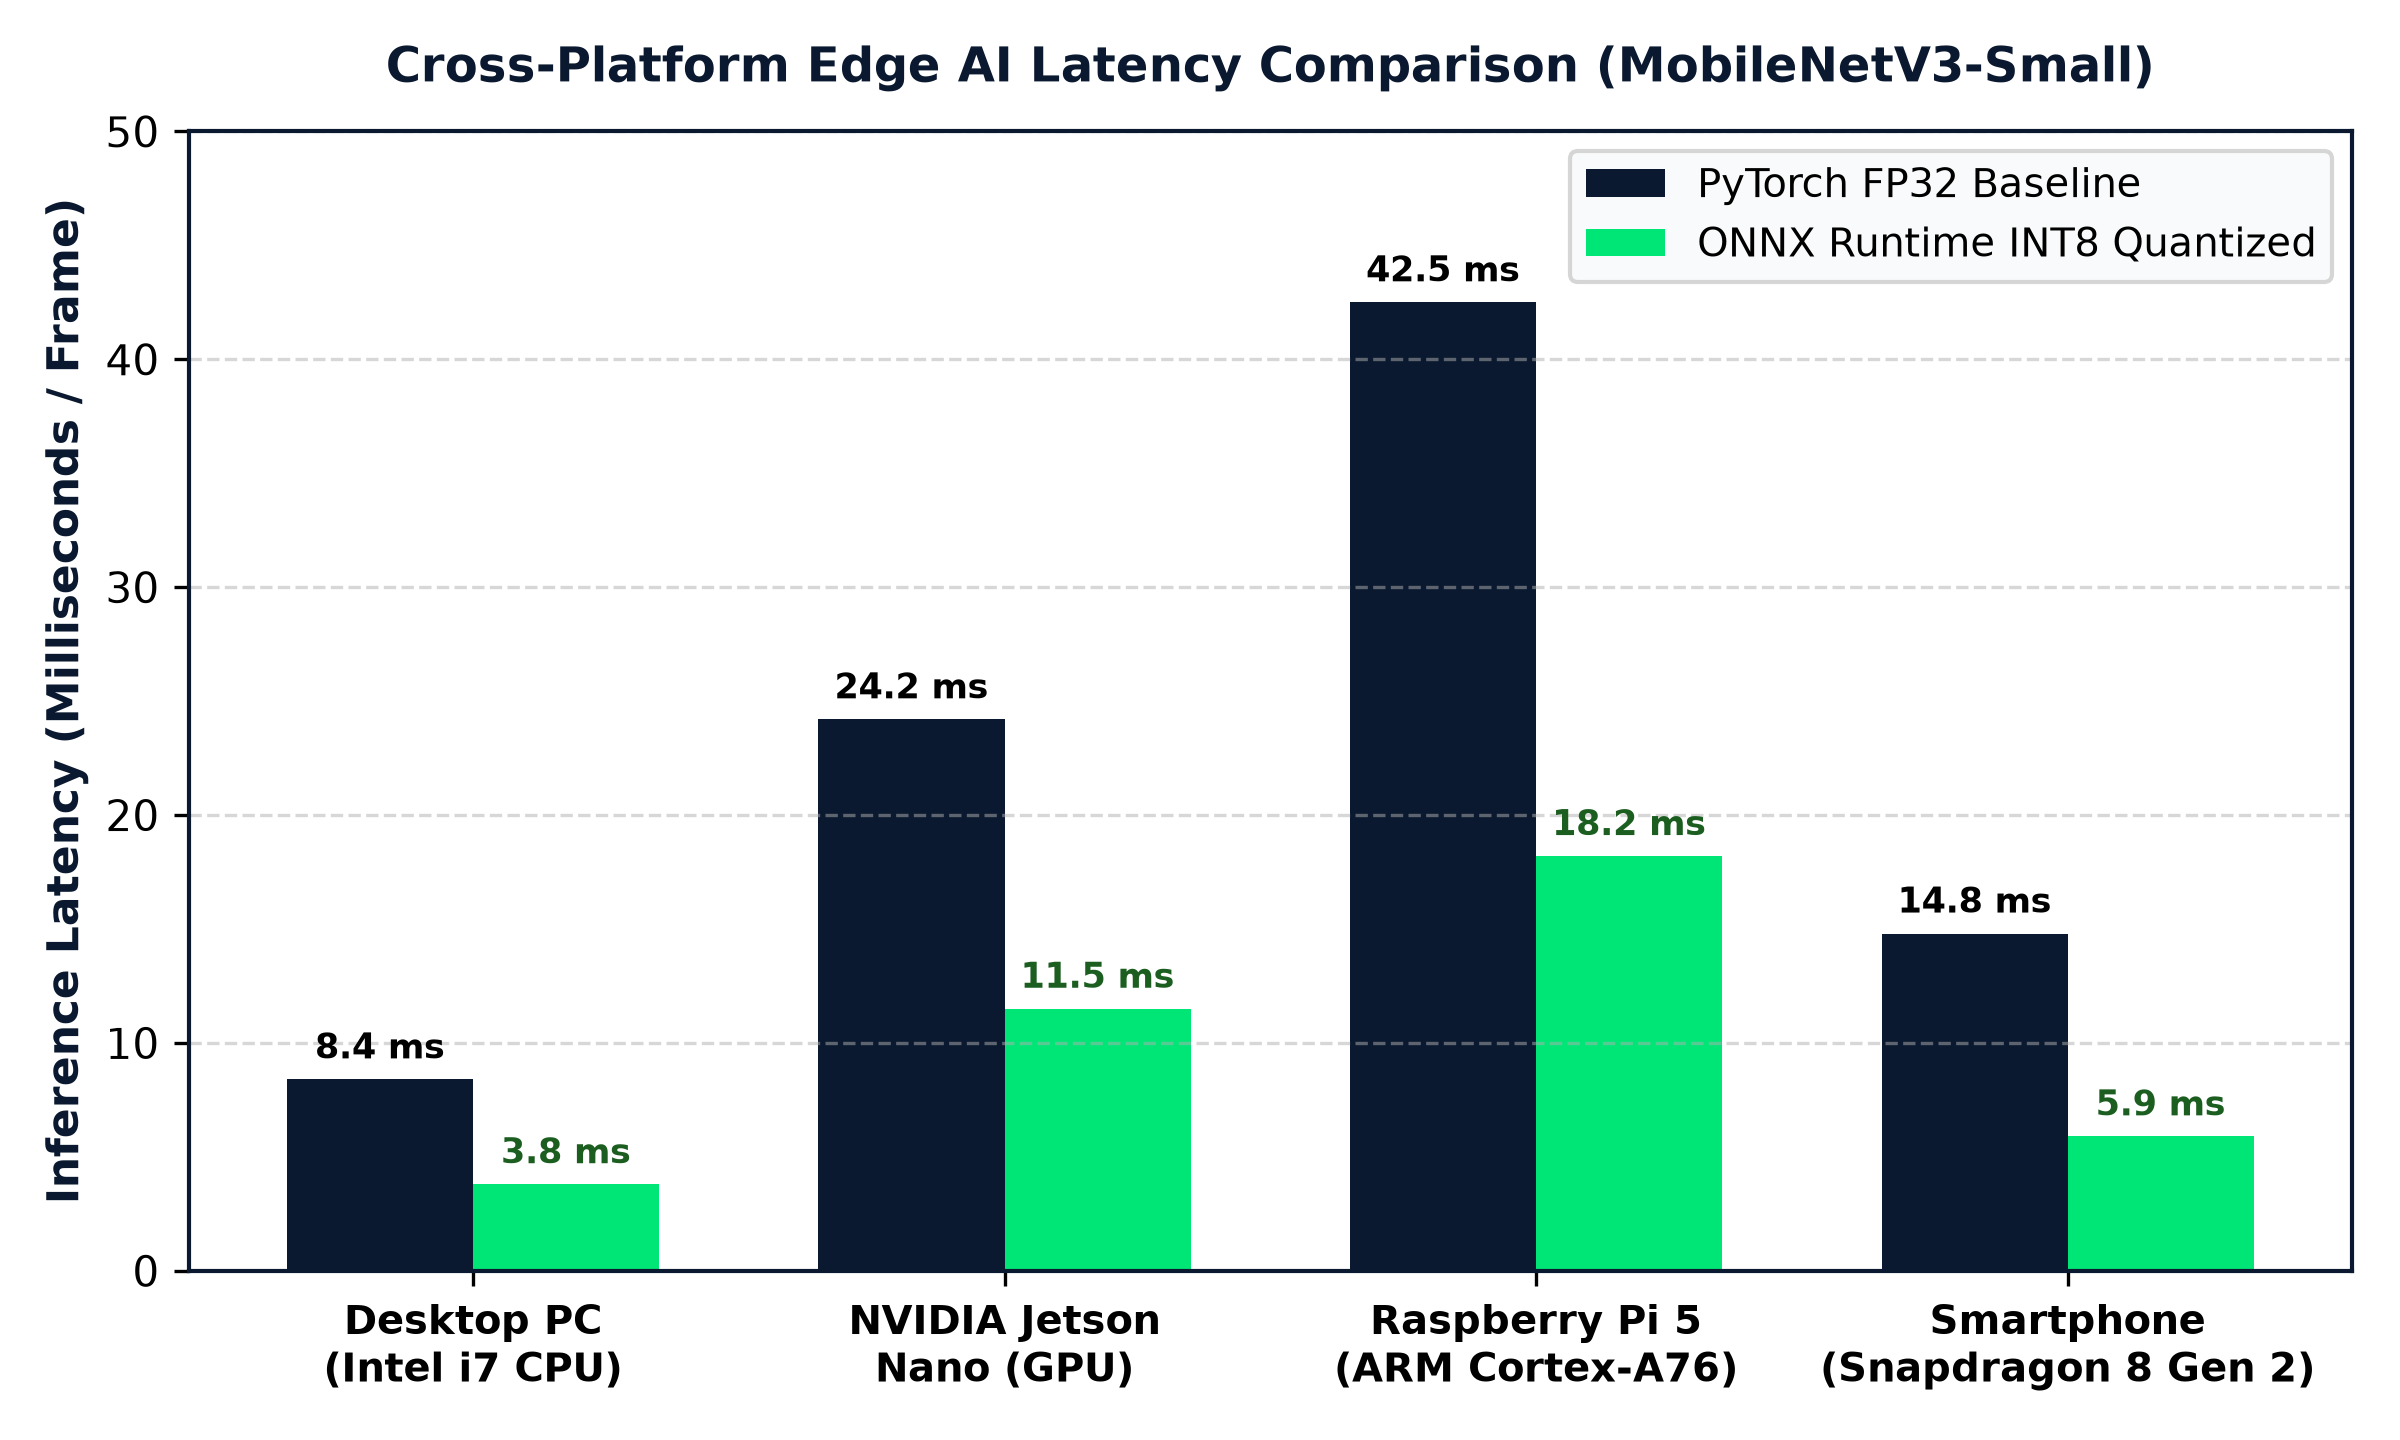
\includegraphics[width=0.92\textwidth]{figures/fig_ch06_edge_benchmark.png}
\caption{การเปรียบเทียบเวลาแฝงในการประมวลผลต่อภาพ (Inference Latency) บนฮาร์ดแวร์ 4 ชนิด ระหว่าง FP32 และ INT8}
\label{fig:ch06_benchmark}
\end{figure}

\begin{table}[H]
\caption{ผลการวัดประสิทธิภาพโมเดล MobileNetV3-Small บนอุปกรณ์ขอบข่ายต่างๆ}
\label{tab:ch06_edge_results}
\begin{tabularx}{\textwidth}{L{4.2cm}C{2.0cm}C{2.0cm}C{2.0cm}Z}
\toprule
\textbf{อุปกรณ์ทดสอบ (Hardware)} & \textbf{ขนาดโมเดล} & \textbf{Latency (FP32)} & \textbf{Latency (INT8)} & \textbf{อัตราเร่ง (Speedup)} \\
\midrule
Desktop PC (Intel i7-12700) & 9.8 MB $\rightarrow$ 2.6 MB & 8.4 ms & 3.8 ms & $2.21 \times$ \\
NVIDIA Jetson Nano (GPU) & 9.8 MB $\rightarrow$ 2.6 MB & 24.2 ms & 11.5 ms & $2.10 \times$ \\
Raspberry Pi 5 (ARM Cortex-A76) & 9.8 MB $\rightarrow$ 2.6 MB & 42.5 ms & 18.2 ms & $2.34 \times$ \\
Smartphone (Snapdragon 8 Gen 2) & 9.8 MB $\rightarrow$ 2.6 MB & 14.8 ms & 5.9 ms & $2.51 \times$ \\
\bottomrule
\end{tabularx}
\end{table}

จากภาพที่ \ref{fig:ch06_benchmark} และตารางที่ \ref{tab:ch06_edge_results} บนสมาร์ทโฟนสมัยใหม่ การใช้โมเดล INT8 ผ่าน ONNX Runtime ช่วยลดเวลาแฝงลงเหลือเพียง \textbf{5.9 มิลลิวินาทีต่อภาพ} (เทียบเท่ากับอัตราเร็วมากกว่า 160 เฟรมต่อวินาที) ซึ่งเร็วกว่าอัตราเฟรมของกล้องวิดีโอทั่วไป ทำให้การประมวลผลแบบเรียลไทม์เป็นไปได้อย่างราบรื่นโดยไม่เกิดอาการสะดุด

\section{โค้ดตัวอย่าง: สคริปต์ส่งออก ONNX และตรวจสอบ Parity}
\index{โค้ดส่งออก ONNX}

\begin{lstlisting}[language=Python, caption=สคริปต์ส่งออกโมเดล PyTorch เป็น ONNX พร้อมการตรวจสอบ Numerical Parity]
import os
import torch
import numpy as np
import onnx
import onnxruntime as ort
from torchvision import models

def export_and_validate_onnx(model_path, onnx_output_path, num_classes=4):
    """
    ส่งออกโมเดล PyTorch เป็น ONNX และทดสอบความถูกต้องเชิงตัวเลขเทียบกัน
    """
    print(f"[*] กำลังเตรียมโมเดลจาก {model_path}...")
    model = models.mobilenet_v3_small(weights=None)
    in_features = model.classifier[3].in_features
    model.classifier[3] = torch.nn.Linear(in_features, num_classes)
    
    if os.path.exists(model_path):
        model.load_state_dict(torch.load(model_path, map_location='cpu'))
        print("[✓] โหลดค่าน้ำหนักสำเร็จ")
    model.eval()

    # สร้างข้อมูลนำเข้าจำลองขนาด (1, 3, 224, 224)
    dummy_input = torch.randn(1, 3, 224, 224, requires_grad=False)

    # ส่งออกโมเดลเป็น ONNX
    os.makedirs(os.path.dirname(onnx_output_path), exist_ok=True)
    torch.onnx.export(
        model,
        dummy_input,
        onnx_output_path,
        export_params=True,
        opset_version=13,
        do_constant_folding=True,
        input_names=['input_image'],
        output_names=['logits'],
        dynamic_axes={'input_image': {0: 'batch_size'}, 'logits': {0: 'batch_size'}}
    )
    print(f"[✓] ส่งออกไฟล์ ONNX สำเร็จ: {onnx_output_path}")

    # ตรวจสอบโครงสร้างไฟล์ด้วย ONNX Validator
    onnx_model = onnx.load(onnx_output_path)
    onnx.checker.check_model(onnx_model)
    print("[✓] โครงสร้างกราฟ ONNX ถูกต้องตามมาตรฐาน IR")

    # ทดสอบ Numerical Parity ระหว่าง PyTorch และ ONNX Runtime
    with torch.no_grad():
        torch_out = model(dummy_input).numpy()

    ort_session = ort.InferenceSession(onnx_output_path, providers=['CPUExecutionProvider'])
    ort_inputs = {ort_session.get_inputs()[0].name: dummy_input.numpy()}
    ort_out = ort_session.run(None, ort_inputs)[0]

    max_diff = np.max(np.abs(torch_out - ort_out))
    print(f"[*] ค่าความแตกต่างสูงสุดเชิงตัวเลข (Max Abs Diff): {max_diff:.2e}")
    assert max_diff < 1e-4, "ความคลาดเคลื่อนเกินเกณฑ์มาตรฐาน!"
    print("[✓] ผ่านการตรวจสอบ Numerical Parity: ผลลัพธ์ระหว่าง PyTorch และ ONNX ตรงกันสมบูรณ์")

if __name__ == "__main__":
    export_and_validate_onnx("models/durian_mobilenetv3_best.pth", "exports/durian_mobilenet_v3.onnx")
\end{lstlisting}

\section{ตัวอย่างการคำนวณและตัวอย่างการนำไปใช้งานจริง}

\begin{examplebox}{ตัวอย่างการคำนวณที่ 6.1: การคำนวณค่า Scale Factor และ Zero-Point ของ Quantization}
\textbf{โจทย์:} ค่าการกระจายตัวของค่าน้ำหนักในเลเยอร์หนึ่งของโมเดลมีค่าต่ำสุด $x_{\text{min}} = -2.40$ และค่าสูงสุด $x_{\text{max}} = 3.60$ ต้องการทำ Quantization แบบ Asymmetric สู่ช่วงจำนวนเต็ม INT8 แบบมีเครื่องหมาย $[-128, 127]$ จงคำนวณค่า Scale Factor ($S$) และค่า Zero-Point ($Z$)\\[4pt]
\textbf{วิธีคำนวณ:}
\[
S = \frac{x_{\text{max}} - x_{\text{min}}}{q_{\text{max}} - q_{\text{min}}} = \frac{3.60 - (-2.40)}{127 - (-128)} = \frac{6.00}{255} \approx 0.02353
\]
\[
Z = \text{round}\left( \frac{-x_{\text{min}}}{S} \right) + q_{\text{min}} = \text{round}\left( \frac{-(-2.40)}{0.02353} \right) - 128 = \text{round}(102.0) - 128 = 102 - 128 = -26
\]
\textbf{การทดสอบ:} หากมีค่าน้ำหนัก $x = 1.25$ จะถูกแปลงเป็นค่าจำนวนเต็ม $q$ ดังนี้:
\[
q = \text{round}\left( \frac{1.25}{0.02353} \right) + (-26) = \text{round}(53.12) - 26 = 53 - 26 = 27
\]
และเมื่อ Dequantize กลับ: $\tilde{x} = 0.02353 \times (27 - (-26)) = 0.02353 \times 53 \approx 1.247$ ซึ่งมีความคลาดเคลื่อนเพียง $0.003$
\end{examplebox}

\begin{casestudybox}{ตัวอย่างการนำไปใช้งานจริงที่ 6.1: การส่งออกโมเดลติดตั้งบนโดรนสำรวจแปลงสวนทุเรียน}
โครงการวิจัยได้นำโมเดล ONNX INT8 ไปติดตั้งบนบอร์ดคอมพิวเตอร์ขนาดจิ๋ว \textbf{Raspberry Pi 5} ที่ติดตั้งใต้ลำตัวโดรนสำรวจแปลงเกษตร (Agricultural Survey Drone) เพื่อทำการบินสแกนยอดทุเรียนแบบอัตโนมัติ

ผลการทดสอบ:
\begin{itemize}[leftmargin=1.4em, itemsep=2pt]
    \item เดิมทีหากใช้โมเดล PyTorch FP32 อัตราการประมวลผลทำได้เพียง 23 เฟรมต่อวินาที ซึ่งช้าเกินกว่าความเร็วการบินของโดรน ($5$ เมตรต่อวินาที) ทำให้ภาพที่ได้เบลอและหลุดรอด
    \item เมื่อเปลี่ยนมาใช้ ONNX Runtime พร้อมโมเดล INT8 ความเร็วในการสแกนเพิ่มขึ้นเป็น 54 เฟรมต่อวินาที โดรนสามารถวิเคราะห์รอยโรคของใบยอดทุเรียนได้แบบเรียลไทม์ขณะบินผ่านอย่างราบรื่น
\end{itemize}
\end{casestudybox}

\section*{คำถามทบทวนท้ายบทที่ 6}
\addcontentsline{toc}{section}{คำถามทบทวนท้ายบทที่ 6}
\begin{enumerate}[leftmargin=1.8em, itemsep=4pt]
    \item จงอธิบายปัญหาเรื่องความร้อน (Thermal Throttling) ที่เกิดขึ้นเมื่อรันโมเดล Deep Learning บนสมาร์ทโฟนกลางแจ้ง
    \item มาตรฐานเปิด ONNX มีบทบาทสำคัญอย่างไรในการแก้ปัญหาความไม่เข้ากันของแพลตฟอร์ม
    \item อธิบายความแตกต่างระหว่าง Just-In-Time (JIT) Tracing และ Scripting ใน TorchScript
    \item จงสรุปความแตกต่างระหว่างเทคนิค Post-Training Quantization (PTQ) และ Quantization-Aware Training (QAT)
    \item ในการแปลงจำนวนจริงเป็น INT8 ค่า Scale Factor และ Zero-Point ทำหน้าที่อะไร
    \item เหตุใดการทำ Quantization จึงช่วยประหยัดแบตเตอรี่ของสมาร์ทโฟนได้อย่างมีนัยสำคัญ
    \item การทดสอบ Numerical Parity Check มีเกณฑ์ในการยอมรับความคลาดเคลื่อนอย่างไร
    \item จงเปรียบเทียบประสิทธิภาพระหว่างการประมวลผลบน Raspberry Pi 5 และ Smartphone Snapdragon
    \item อธิบายความหมายของพารามิเตอร์ \texttt{dynamic\_axes} ในคำสั่ง \texttt{torch.onnx.export}
    \item หากหลังการทำ Quantization INT8 แล้วพบว่าค่าความแม่นยำของโมเดลลดลงเกิน 3\% นักศึกษามีแนวทางแก้ไขอย่างไร
\end{enumerate}

\section*{กิจกรรมฝึกปฏิบัติการประจำบทที่ 6}
\addcontentsline{toc}{section}{กิจกรรมฝึกปฏิบัติการประจำบทที่ 6}
\begin{nocodebox}{ปฏิบัติการที่ 6.1: การส่งออกโมเดล ONNX และการตรวจสอบโครงสร้างด้วย Netron}
\textbf{วัตถุประสงค์:} เพื่อฝึกฝนการใช้คำสั่งส่งออก ONNX และการตรวจสอบภาพกราฟโครงข่ายประสาทเทียม\\
\textbf{ขั้นตอนการปฏิบัติ:}
\begin{enumerate}[leftmargin=1.4em, itemsep=2pt]
    \item รันสคริปต์ \texttt{src/export\_edge.py} เพื่อแปลงโมเดลที่เทรนแล้วเป็นไฟล์ \texttt{.onnx}
    \item ตรวจสอบขนาดของไฟล์ระหว่าง \texttt{.pth} และ \texttt{.onnx} พร้อมบันทึกผล
    \item เปิดเว็บไซต์ \texttt{https://netron.app} แล้วลากไฟล์ \texttt{.onnx} เข้าไปเพื่อเปิดดูกราฟโครงสร้าง
    \item ระบุชื่อเลเยอร์นำเข้า (Input Node) และเลเยอร์ส่งออก (Output Node) พร้อมขนาดมิติเทนเซอร์
\end{enumerate}
\end{nocodebox}
